\documentclass[10pt,a4paper]{article}

\usepackage[T1]{fontenc}
\usepackage[utf8]{inputenc}
\usepackage{lmodern}
\usepackage[scaled=0.92]{helvet}
\renewcommand{\familydefault}{\sfdefault}
\renewcommand{\ttdefault}{lmtt}
\usepackage[italic]{mathastext}
\usepackage{amsmath,amssymb}
\usepackage{microtype}
\usepackage[a4paper,left=1.75cm,right=1.75cm,top=1.65cm,bottom=1.7cm,headheight=19pt]{geometry}
\usepackage{ragged2e}
\usepackage{booktabs}
\usepackage{tabularx}
\usepackage{array}
\usepackage{enumitem}
\usepackage{listings}
\usepackage[table]{xcolor}
\usepackage{tcolorbox}
\usepackage{tikz}
\usetikzlibrary{arrows.meta,positioning,fit,backgrounds,calc}
\usepackage{titlesec}
\usepackage{fancyhdr}
\usepackage[colorlinks=true,linkcolor=navy,urlcolor=teal,citecolor=teal]{hyperref}
\usepackage[font=small,labelfont=bf,textfont=small]{caption}
\renewcommand{\figurename}{Figura}
\renewcommand{\tablename}{Tabla}

\definecolor{navy}{HTML}{12355B}
\definecolor{teal}{HTML}{0F7B6C}
\definecolor{amber}{HTML}{B9770E}
\definecolor{crimson}{HTML}{A33A32}
\definecolor{ink}{HTML}{1F2933}
\definecolor{mist}{HTML}{F2F5F7}
\definecolor{slate}{HTML}{5B6770}

\color{ink}
\RaggedRight
\setlength{\parindent}{0pt}
\setlength{\parskip}{2.2pt}
\renewcommand{\arraystretch}{1.12}
\setlist[itemize]{leftmargin=1.05em,itemsep=1.2pt,topsep=2pt,parsep=0pt}
\setlist[enumerate]{leftmargin=1.25em,itemsep=1.2pt,topsep=2pt,parsep=0pt}

\titleformat{\section}{\large\bfseries\color{navy}}{\thesection.}{0.45em}{}
\titlespacing*{\section}{0pt}{7pt plus 2pt minus 1pt}{2pt}
\titleformat{\subsection}{\normalsize\bfseries\color{teal}}{\thesubsection}{0.45em}{}
\titlespacing*{\subsection}{0pt}{5pt plus 1pt minus 1pt}{1pt}
\titleformat{\paragraph}[runin]{\normalsize\bfseries\color{navy}}{}{0pt}{}[\hspace{0.4em}]
\titlespacing*{\paragraph}{0pt}{3pt}{0.4em}

\pagestyle{fancy}
\fancyhf{}
\fancyhead[L]{\footnotesize\bfseries\color{navy}Xplainable}
\fancyhead[R]{\footnotesize\color{slate}Documento técnico · More than a Hack 2027}
\fancyfoot[C]{\footnotesize\color{slate}\thepage}
\renewcommand{\headrulewidth}{0.35pt}
\renewcommand{\headrule}{\hbox to\headwidth{\color{navy!35}\leaders\hrule height \headrulewidth\hfill}}

\lstset{
  basicstyle=\ttfamily\footnotesize,
  backgroundcolor=\color{mist},
  frame=none,
  breaklines=true,
  columns=fullflexible,
  keepspaces=true,
  showstringspaces=false,
  aboveskip=2pt,
  belowskip=2pt,
  xleftmargin=3pt,
  xrightmargin=3pt
}

\newcommand{\good}[1]{\textcolor{teal}{\bfseries #1}}
\newcommand{\bad}[1]{\textcolor{crimson}{\bfseries #1}}
\newcommand{\code}[1]{\texttt{\small #1}}
\newcommand{\sha}[1]{\texttt{\scriptsize #1}}

\hypersetup{
  pdftitle={Xplainable - Posesi\'on fotograma a fotograma},
  pdfauthor={Equipo Xplainable},
  pdfsubject={More than a Hack 2027 - Fase 1: Posesi\'on},
  pdfkeywords={HMM, posesi\'on, f\'utbol, tracking, YOLO, spellF1}
}

\begin{document}
\thispagestyle{empty}

% ----------------------------------------------------------------------------- title
\begin{tcolorbox}[colback=white, colframe=white, boxrule=0pt, left=0pt, right=0pt, top=0pt, bottom=0pt]
{\footnotesize\bfseries\color{teal}MORE THAN A HACK 2027 \textperiodcentered{} FASE 1: POSESIÓN}\\[3pt]
{\fontsize{30}{32}\selectfont\bfseries\color{navy}Xplainable}\\[2pt]
{\Large\color{ink}Posesión fotograma a fotograma sobre tracking táctico}\\[5pt]
{\small\color{slate}FC Barcelona -- Athletic Club \textperiodcentered{} 199.319 fotogramas \textperiodcentered{} 25 fps \textperiodcentered{} 105,3 $\times$ 68,0 m \textperiodcentered{} 17 de noviembre de 2026}
\end{tcolorbox}

\vspace{-2pt}
{\color{navy!30}\rule{\textwidth}{0.7pt}}
\vspace{2pt}

\begin{center}
\begin{tabular}{@{}c@{\hspace{2.1cm}}c@{\hspace{2.1cm}}c@{\hspace{2.1cm}}c@{}}
{\fontsize{19}{20}\selectfont\bfseries\color{navy}0,9257} &
{\fontsize{19}{20}\selectfont\bfseries\color{navy}0,9661} &
{\fontsize{19}{20}\selectfont\bfseries\color{navy}18 / 17} &
{\fontsize{19}{20}\selectfont\bfseries\color{navy}199.319}\\[-1pt]
{\footnotesize\color{slate}spellF1 público} &
{\footnotesize\color{slate}macroF1 (H/A/D)} &
{\footnotesize\color{slate}posesiones predichas / GT} &
{\footnotesize\color{slate}filas del CSV}
\end{tabular}
\end{center}
\vspace{-1pt}

% ----------------------------------------------------------------------------- resumen
\section{Resumen y enfoque}

El objetivo es asignar a cada uno de los 199.319 fotogramas del partido uno de cuatro estados:
\good{H} (posesión del Barcelona), \good{A} (Athletic Club), \good{D} (balón muerto o fuera de
juego) o \good{X} (abstención). El envío es un único CSV de 199.319 filas que produce una cadena
determinista, sin etiquetas manuales y sin usar la verdad privada. La dificultad no es acertar el
fotograma medio: es \emph{no fragmentar las posesiones}. La métrica que decide la clasificación,
\texttt{spellF1}, empareja posesiones completas; un cambio espurio de un segundo puede destruir
una posesión correcta de treinta.

Nuestro punto de partida es el ATD táctico: 46 slots anónimos, sin identidad de jugador, y el
balón observado sólo en el \textbf{56,9\,\%} de los fotogramas (2,2\,\% estimado y 40,8\,\% sin
ninguna estimación). Sobre esa base construimos tres capas. Primero, un \textbf{HMM de tres
estados} con persistencia fuerte, emisiones geométricas y un modelo explícito de huecos. Segundo,
una \textbf{capa de percepción} con dos detectores YOLO26x (balón y jugadores) y un \textbf{poll
log-opinion} que incorpora evidencia independiente sin sustituir al HMM. Tercero, una
\textbf{capa de transiciones} dirigida por eventos físicos ---kicks, controles y contactos--- que
es la que convierte un seguimiento suave en posesiones correctas.

La razón de este diseño es doble. Con sólo cinco minutos de verdad pública, un modelo extremo a
extremo aprendería a copiar esa ventana; en cambio, un HMM auditable más reglas físicas se puede
verificar, ejecutar en CPU y reproducir byte a byte. Y la literatura de posesión coincide con la
intuición: los cambios de posesión son eventos discretos (un golpeo, un control, una intercepción),
no una deriva continua de distancias. El HMM aporta estabilidad; los eventos aportan el instante.

En la ventana pública (7.500 fotogramas, 17 posesiones) el HMM con fusión obtiene
\textbf{0,6519} de spellF1. La capa de transiciones sube a \textbf{0,9257}, con macroF1
\textbf{0,9661} y accuracy \textbf{0,9689}. El intervalo bootstrap del 95\,\% para spellF1 es
[0,857; 0,971]: con 17 posesiones es ancho, y no debe leerse una diferencia pequeña como una
mejora real.

\begin{center}
\small
\captionof{table}{Ventana pública de evaluación: fotogramas 11.185--18.684 (7.500), 17 posesiones GT
y 14,2 s de duración media. La columna derecha es el fichero enviado. El bootstrap usa 2.000
remuestreos.}
\label{tab:metrics}
\begin{tabular}{lrr}
\toprule
Métrica & HMM + fusión & \textbf{+ transiciones} \\
\midrule
spellF1 (principal) & 0,6519 & \textbf{0,9257} \\
spellF1 con IoU 0,5 & 0,6667 & 0,9143 \\
macroF1 (H/A/D) & 0,9469 & \textbf{0,9661} \\
accuracy & 0,9420 & 0,9689 \\
kappa de Cohen & 0,9087 & 0,9507 \\
F1 de la clase D & 0,9733 & 0,9574 \\
team accuracy (ambos vivos) & 0,9405 & 0,9815 \\
posesiones predichas & 10 & 18 \\
duración media de posesión & 24,0 s & 13,6 s \\
bootstrap 95\,\% de spellF1 & [0,430; 0,817] & [0,857; 0,971] \\
\bottomrule
\end{tabular}
\end{center}

La capa de transiciones baja ligeramente el F1 de D (0,9733 $\to$ 0,9574) porque convierte algunos
fotogramas de \emph{balón muerto} cercanos al evento en la posesión del equipo que lo provoca. Es
un intercambio deliberado: el spellF1 sube 27,4 puntos y el macroF1 también mejora. El resto de
esta nota explica cómo se toma cada decisión y dónde falla.

% ----------------------------------------------------------------------------- arquitectura
\section{Arquitectura}

La figura~\ref{fig:arch} muestra la cadena completa. Los activos entran una sola vez; cada capa
produce un artefacto intermedio verificable. La percepción es la única etapa que necesita GPU;
fusión, transiciones, explicador y visor son CPU determinista.

\begin{figure}[t]
\centering
\begin{tikzpicture}[
  font=\scriptsize,
  input/.style={draw=slate!55, fill=mist, rounded corners=1.5pt, align=center, inner sep=2.4pt, minimum height=8.5mm, text width=2.8cm},
  model/.style={draw=teal!85!black, fill=teal!8, rounded corners=2pt, align=center, inner sep=3pt, minimum height=11mm, text width=5.1cm},
  wide/.style={draw=navy, fill=navy!6, rounded corners=2pt, align=center, inner sep=3pt},
  inner/.style={draw=amber!85!black, fill=amber!10, rounded corners=1.5pt, align=center, inner sep=2.2pt, text width=3.75cm, minimum height=10mm},
  output/.style={draw=navy, fill=navy!12, rounded corners=2pt, align=center, inner sep=3pt, minimum height=10mm, text width=5.5cm},
  arr/.style={-{Latex[length=1.5mm]}, draw=slate!70, line width=0.55pt},
  bus/.style={draw=slate!70, line width=0.7pt}
]
% inputs
\node[input] (atd) at (2.0,0)  {\textbf{ATD táctico}\\balón + 46 slots};
\node[input] (tags) at (5.2,0) {\textbf{Smart tags}\\638 intervalos};
\node[input] (hom) at (8.4,0)  {\textbf{Homografía}\\105,3 $\times$ 68,0 m};
\node[input] (aud) at (11.6,0){\textbf{Audio MP4}\\silbato 2,4--3,8 kHz};
\node[input] (vid) at (14.8,0){\textbf{Vídeo táctico}\\199.319 fotogramas};
\node[font=\scriptsize\bfseries, text=navy, anchor=south west] at (0.0,0.62) {ACTIVOS DE ENTRADA};
% bus
\draw[bus] (0.25,-1.18) -- (16.55,-1.18);
\foreach \n in {atd,tags,hom,aud,vid} \draw[arr] (\n.south) -- ++(0,-0.28);
% models
\node[model] (hmm) at (4.5,-2.65) {\textbf{HMM base (ATD)}\\emisiones $q_H,q_A,q_D$ \textperiodcentered{} Viterbi\\persistencia $p_{stay}=0{,}995$};
\node[model] (yolo) at (11.5,-2.65) {\textbf{Percepción YOLO26x}\\balón + jugadores a 1024 px\\compuerta física 40 m/s $+$ 1 m};
\draw[arr] (4.5,-1.18) -- (hmm.north);
\draw[arr] (11.5,-1.18) -- (yolo.north);
% poll
\node[wide, text width=14.5cm, minimum height=9mm] (poll) at (8.4,-4.55)
  {\textbf{Poll multi-fuente (8 votantes):} HMM 1,00 \textperiodcentered{} YOLO balón 0,10 \textperiodcentered{} jugadores 0,10 \textperiodcentered{} ATD 0,02/0,01 \textperiodcentered{} tags 0,01 \textperiodcentered{} audio 0,02 \textperiodcentered{} eventos 1,00 (D duro)};
\draw[arr] (hmm.south) -- ++(0,-0.3) -| ([xshift=-2.6cm]poll.north);
\draw[arr] (yolo.south) -- ++(0,-0.3) -| ([xshift=2.6cm]poll.north);
% transition layer
\node[wide, text width=14.5cm, minimum height=20mm] (transbg) at (8.4,-7.02) {};
\node[font=\scriptsize\bfseries, text=navy, anchor=north] at (8.4,-6.05) {CAPA DE TRANSICIONES (eventos $\rightarrow$ posesiones)};
\node[inner] (det) at (3.35,-7.28) {\textbf{1 \textperiodcentered{} Detectar}\\kicks, onsets, contactos\\y manos del portero};
\node[inner] (gate) at (8.4,-7.28) {\textbf{2 \textperiodcentered{} Filtrar}\\equipo distinto, balón vivo\\evidencia $\geq 0{,}10$ durante 2 s};
\node[inner] (rede) at (13.45,-7.28) {\textbf{3 \textperiodcentered{} Re-decodificar}\\pulso logit + Viterbi\\+ reglas de reanudación};
\draw[arr] (poll.south) -- (transbg.north);
% outputs
\node[output] (csv) at (4.6,-9.35) {\textbf{Xplainable.csv}\\199.319 filas \textperiodcentered{} H/A/D/X};
\node[output, draw=amber!85!black, fill=amber!8] (view) at (12.2,-9.35) {\textbf{Explicador + visor}\\por qué cambia cada posesión};
\draw[arr] (transbg.south) -- ++(0,-0.25) -| ([xshift=-1.5cm]csv.north);
\draw[arr] (transbg.south) -- ++(0,-0.25) -| ([xshift=1.5cm]view.north);
\end{tikzpicture}
\caption{Arquitectura en cuatro etapas. La percepción y el HMM producen votos independientes;
el poll los pondera con el HMM como ancla; la capa de transiciones detecta eventos, los filtra y
re-decodifica. La verdad pública sólo se usa en la evaluación (no aparece en la figura porque no
es una entrada).}
\label{fig:arch}
\end{figure}

\paragraph{Activos.} El ATD aporta el balón y 46 slots (24 Barcelona, 22 Athletic) en metros, a
25 fps, con $x=0$ en la portería del Barcelona. Los smart tags aportan 638 intervalos y 14 códigos
(tipos de reanudación, progresión, ocasión, gol); los saques de banda llegan sin equipo. La
homografía se usa para diagnosticar la validez y para proyectar el visor, nunca como etiqueta. El
audio del MP4 alimenta el detector de silbato. El vídeo táctico alimenta la percepción YOLO.

\paragraph{Percepción.} Dos detectores YOLO26x a 1024 px, entrenados \emph{sólo} con datos
externos, producen cajas de jugador y balón. Los pies se proyectan a metros con la homografía;
el equipo de cada jugador se toma del slot ATD más cercano (no se afirma identidad ni color de
camiseta). Una compuerta física de $40\ \mathrm{m/s}+1\ \mathrm{m}$ rechaza detecciones
inalcanzables, y adquirir o readquirir una pista exige dos detecciones mutuamente alcanzables. El
tracker propio se ancla al ATD mientras éste ve el balón y sólo acepta medidas de vídeo dentro de
la compuerta; si no tiene ni ancla ni medida, declara \emph{perdido}. En la ventana pública se
aceptaron 4.497 observaciones YOLO: la detección cruda tenía 566 saltos por encima de 2,6 m por
fotograma (máximo 84,9 m); tras la compuerta, ningún par consecutivo la supera (máximo 1,86 m).

\paragraph{Fusión.} Cada fuente emite una probabilidad sobre H/A/D. El poll es una mezcla
log-opinion anclada en el HMM:
\begin{equation}
\log p \;\propto\; w_{\mathrm{hmm}}\log q_{\mathrm{hmm}}
\;+\;\sum_i w_i \log p_i,
\qquad w_{\mathrm{hmm}}=1{,}00 .
\label{eq:pool}
\end{equation}
Los pesos son un prior de diseño, no se ajustaron con la verdad. ATD, tags y audio pesan poco
porque ya están dentro de la emisión del HMM; contarlos otra vez sería duplicar evidencia. YOLO y
los jugadores YOLO son la evidencia independiente. Los eventos confirmados son un $D$ duro. Tras
el poll, un HMM temporal con el mismo prior decodifica la secuencia. La fusión por sí sola no
mejora el spellF1 (0,6519): es una capa de seguridad y de evidencia para la etapa siguiente, no
un sustituto del HMM.

\paragraph{Transiciones.} Es la capa que aporta la ganancia. El poll es un suavizador: el HMM
concentra unas 2,7 nats de evidencia temporal y los votos de evidencia suman menos de 0,5 nats,
así que un cambio real de un solo fotograma se decodifica tarde o se pierde. La capa detecta
el evento físico, lo atribuye a un equipo, comprueba que la evidencia independiente lo respalda y
re-decodifica con un pulso decreciente en el logit del equipo entrante, una matriz de transición
relajada alrededor del evento y protección para que el suavizado posterior no absorba el hechizo.
Sobre el partido completo se detectaron 194 kicks y 23 onsets; las compuertas descartaron 1.004
candidatos y se conservaron 100 eventos.

% ----------------------------------------------------------------------------- modelos
\section{Modelos}

\subsection{HMM base: estabilidad y huecos}

El HMM tiene tres estados y cuatro probabilidades de transición deliberadamente pegajosas:
\begin{equation}
p_{stay}=0{,}995,\qquad p_{ha}=0{,}0005,\qquad p_{hd}=0{,}001,\qquad p_{dh}=0{,}007,
\label{eq:trans}
\end{equation}
La fila de D cierra con $1-2p_{dh}=0{,}986$. Con el balón visible, la emisión compara la distancia del balón al jugador más cercano de cada
equipo, con $\sigma=4{,}0$ m:
\begin{equation}
q_H=e^{-d_H^2/(2\sigma^2)},\qquad
q_A=e^{-d_A^2/(2\sigma^2)},\qquad
q_D=\operatorname{sigmoide}\!\left(\frac{\min(d_H,d_A)-8{,}0}{1{,}5}\right)+\cdots
\label{eq:emis}
\end{equation}
La parte $q_D$ suma evidencia independiente de balón muerto: balón fuera del campo, balón parado
junto a una línea, energía de movimiento del equipo y el patrón de balón aparcado en la banda. Si
el balón está a más de 7 m de todos los jugadores se considera suelto o en vuelo y la emisión es
uniforme; si además va a menos de 2 m/s, el último equipo que lo tocó recibe el 70\,\% de la masa
cuando el toque tiene menos de 5 s. Para huecos de hasta 120 fotogramas (4,8 s) la emisión es
uniforme; en huecos más largos se usa la forma del equipo alrededor de la última posición conocida
y la distancia a la línea, con un prior débil. Con menos de 6 jugadores visibles se trata como
evidencia ausente, no como un equipo.

El decode es un Viterbi por mitad con 500 fotogramas de contexto. Las mitades puntuadas son
[11.185, 90.652) y [110.808, 190.198); el resto no se evalúa, y la capa final lo rellena con D
salvo el prepartido y el final, que quedan como X. Después se absorben los tramos de menos de 1 s que vuelven a la etiqueta
anterior: un parpadeo de tracking no es un cambio de posesión. Los goles y las paradas confirmadas
se aplican como un $D$ duro \emph{después} del Viterbi. En el partido completo se confirmaron dos
goles (46.691 por trayectoria y 157.825 por celebración) y 68 paradas; los intervalos de gol se
extienden hasta la reanudación.

\begin{figure}[t]
\centering
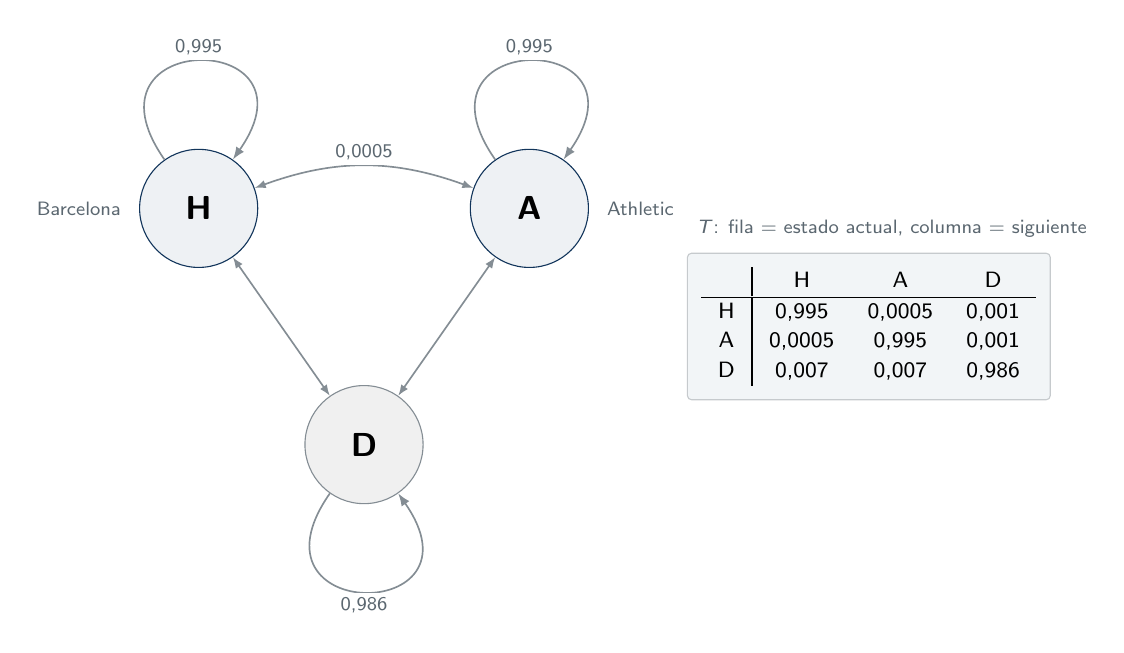
\begin{tikzpicture}[
  font=\scriptsize,
  state/.style={circle, draw=navy, fill=navy!7, minimum size=15mm, inner sep=0pt, font=\large\bfseries},
  dstate/.style={circle, draw=slate!75, fill=gray!12, minimum size=15mm, inner sep=0pt, font=\large\bfseries},
  edge/.style={-{Latex[length=1.6mm]}, draw=slate!75, line width=0.6pt},
  bi/.style={draw=slate!75, line width=0.6pt, {Latex[length=1.4mm]}-{Latex[length=1.4mm]}},
  lbl/.style={font=\scriptsize, text=slate, inner sep=2pt, fill=white}
]
\node[state] (H) at (0,0) {H};
\node[state] (A) at (4.2,0) {A};
\node[dstate] (D) at (2.1,-3.0) {D};
\node[font=\scriptsize, text=slate, left=3pt of H] {Barcelona};
\node[font=\scriptsize, text=slate, right=3pt of A] {Athletic};
% self loops
\draw[edge] (H) to[out=125,in=55,looseness=6] node[lbl,above]{$0{,}995$} (H);
\draw[edge] (A) to[out=125,in=55,looseness=6] node[lbl,above]{$0{,}995$} (A);
\draw[edge] (D) to[out=235,in=305,looseness=6] node[lbl,below]{$0{,}986$} (D);
% cross edges (numeric values in the matrix panel)
\draw[bi] (H) to[bend left=20] node[lbl,above]{$0{,}0005$} (A);
\draw[bi] (H) -- (D);
\draw[bi] (A) -- (D);
% transition matrix
\node[draw=slate!35, fill=mist, rounded corners=1.5pt, inner sep=5pt, anchor=west, font=\footnotesize] (mat) at (6.2,-1.5) {%
  \begin{tabular}{c|ccc}
   & H & A & D\\ \hline
  H & $0{,}995$ & $0{,}0005$ & $0{,}001$\\
  A & $0{,}0005$ & $0{,}995$ & $0{,}001$\\
  D & $0{,}007$ & $0{,}007$ & $0{,}986$
  \end{tabular}};
\node[font=\scriptsize, text=slate, anchor=south west] at ([yshift=2pt]mat.north west)
  {$T$: fila = estado actual, columna = siguiente};
\end{tikzpicture}
\caption{El HMM base. La matriz $T$ (filas: estado actual; columnas: siguiente) y los autolazos
gobiernan la persistencia. La emisión geométrica usa $\sigma=4{,}0$ m y $d_{dead}=8{,}0$ m; el
decode es un Viterbi por mitad con 500 fotogramas de contexto. La persistencia ($p_{stay}=0{,}995$)
evita fragmentar; la salida de D es algo más fácil ($p_{dh}=0{,}007$) porque las paradas
confirmadas ya están garantizadas por la capa de eventos.}
\label{fig:hmm}
\end{figure}

\subsection{Percepción: una segunda mirada, con freno físico}

El ATD no observa el balón en el 43,1\,\% del partido (2,2\,\% estimado y 40,8\,\% sin
estimación). La percepción no sustituye al ATD: produce
una \emph{segunda} observación del vídeo para los fotogramas en los que el tracking táctico no
basta. Los dos detectores son YOLO26x a 1024 px, entrenados con SoccerNet v3 H250 (CC-BY-4.0),
el dataset público de infactory-ai (CC-BY-NC-4.0) y el de martinjolif (CC-BY-4.0) para el balón, y
SoccerNet/SN-Tracking-2023, martinjolif (jugadores, CC-BY-4.0), keremberke (CC-BY-4.0) y manot
(MIT) para jugadores; los nombres completos están en \texttt{REPRODUCING.md}. Ningún fotograma de
este partido ni ninguna etiqueta de posesión entraron en el entrenamiento.

La compuerta es cinemática, no una consulta a la verdad: el balón no puede recorrer más de
$40\ \mathrm{m/s}\cdot\Delta t + 1\ \mathrm{m}$ entre dos observaciones aceptadas. Una detección
fuera de ese radio se descarta aunque el detector esté muy seguro; una predicción de velocidad no
ensancha la compuerta, porque el candidato debe ser alcanzable desde el último punto aceptado, no
sólo desde la posición predicha. La readquisición exige dos detecciones mutuamente alcanzables.
El tracker propio se ancla al ATD y, en un hueco, sólo acepta medidas dentro de la compuerta; si
no tiene ni ancla ni medida, no inventa una posición.

\subsection{Fusión: ocho votantes y un ancla}

La tabla~\ref{tab:weights} resume el poll. Cada fuente emite una distribución sobre H/A/D y el
peso efectivo se reduce además por su calidad (confianza del balón, cobertura de jugadores, edad
de la muestra, si el ATD ya ve el balón). El HMM es el ancla; las demás fuentes tienen que ganar
la discrepancia, no reemplazarla por decreto.

\begin{table}[t]
\centering
\small
\caption{Votantes del poll y pesos base. Los pesos son un prior de diseño; no se ajustaron con la
verdad pública. El HMM aporta 1,00 y cada evidencia se suma como una actualización de
verosimilitud en el logit.}
\label{tab:weights}
\begin{tabular}{llr}
\toprule
Fuente & Papel & Peso \\
\midrule
HMM ATD & ancla / prior temporal & 1,00 \\
YOLO balón & evidencia independiente & 0,10 \\
Jugadores YOLO & evidencia independiente & 0,10 \\
ATD balón & diagnóstico (ya está en la emisión) & 0,02 \\
ATD forma & diagnóstico & 0,01 \\
Smart tags & diagnóstico & 0,01 \\
Silbato & diagnóstico & 0,02 \\
Eventos & $D$ duro (goles, paradas) & 1,00 \\
\bottomrule
\end{tabular}
\end{table}

\subsection{Transiciones: del suavizado al evento}

Un kick se detecta cuando el balón gana al menos 6 m/s y sale a 8--32 m/s hacia un jugador que
está a menos de 2 m; un \emph{onset} de control se detecta cuando un balón que iba a 7 m/s o más
se mata a 4 m/s o menos junto a un jugador que venía siendo perseguido. Ambos se atribuyen al
equipo del jugador más cercano, con supresión no máxima por equipo. La capa de píxeles añade
contactos dentro de la caja del jugador, kicks de despeje y manos del portero; la geometría de
área añade la cogida del portero cuando el balón muere dentro de su área.

Un evento sólo se convierte en transición si se cumplen todas las condiciones: el equipo
atribuido es distinto del poseedor actual; el balón está vivo (sin hueco del ATD ni ventana de
balón muerto); el equipo atribuido estaba en el balón al menos 8 de los 15 fotogramas anteriores;
la evidencia independiente favorece al equipo atribuido frente al actual con un margen medio de
al menos 0,10 durante los 2 s siguientes; y el balón sigue vivo en la ventana. Entonces se aplica
un pulso logit decreciente al equipo entrante, se relaja la matriz de transición alrededor del
evento y se protege el hechizo para que el merge de flickers no lo absorba.

\begin{figure}[t]
\centering
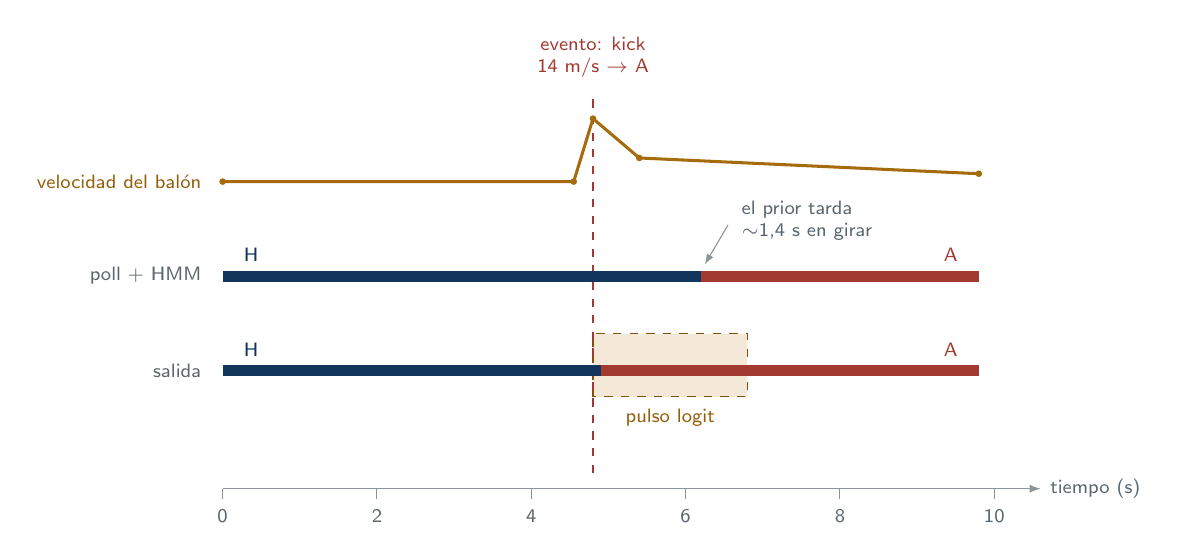
\begin{tikzpicture}[font=\scriptsize, x=0.98cm, y=1cm]
% pulse shading (behind the bands)
\fill[amber!16] (4.8,0.62) rectangle (6.8,1.42);
\draw[amber!70!black, dashed] (4.8,0.62) rectangle (6.8,1.42);
% time axis
\draw[-{Latex[length=1.4mm]}, slate!70] (0,-0.55) -- (10.6,-0.55) node[right, text=slate]{tiempo (s)};
\foreach \t in {0,2,4,6,8,10} {
  \draw[slate!70] (\t,-0.55) -- (\t,-0.68);
  \node[text=slate, anchor=north] at (\t,-0.7) {\t};
}
% event line
\draw[dashed, crimson, line width=0.8pt] (4.8,-0.35) -- (4.8,4.5);
\node[crimson, anchor=south, align=center] at (4.8,4.55) {evento: kick\\14 m/s $\to$ A};
% ball speed
\draw[line width=1.1pt, amber!90!black] (0,3.35) -- (4.55,3.35) -- (4.8,4.15) -- (5.4,3.65) -- (9.8,3.45);
\foreach \p in {(0,3.35),(4.55,3.35),(4.8,4.15),(5.4,3.65),(9.8,3.45)} \fill[amber!90!black] \p circle (1.2pt);
\node[anchor=east, text=amber!80!black] at (-0.15,3.35) {velocidad del balón};
% poll band
\draw[line width=4pt, navy] (0,2.15) -- (6.2,2.15);
\draw[line width=4pt, crimson] (6.2,2.15) -- (9.8,2.15);
\node[navy, anchor=west] at (0.15,2.42) {H};
\node[crimson, anchor=east] at (9.65,2.42) {A};
\node[anchor=east, text=slate] at (-0.15,2.15) {poll + HMM};
% final band
\draw[line width=4pt, navy] (0,0.95) -- (4.9,0.95);
\draw[line width=4pt, crimson] (4.9,0.95) -- (9.8,0.95);
\node[navy, anchor=west] at (0.15,1.22) {H};
\node[crimson, anchor=east] at (9.65,1.22) {A};
\node[anchor=east, text=slate] at (-0.15,0.95) {salida};
% annotations
\draw[-{Latex[length=1.3mm]}, slate!70] (6.55,2.8) -- (6.25,2.3);
\node[anchor=west, align=left, text=slate] at (6.6,2.85) {el prior tarda\\$\sim$1,4 s en girar};
\node[text=amber!80!black, anchor=north] at (5.8,0.58) {pulso logit};
\end{tikzpicture}
\caption{Anatomía conceptual de una transición. El evento (línea roja) es inmediato; el poll con
inercia HMM tarda en girar; el pulso y la relajación de la matriz mueven la frontera al evento y
protegen el hechizo. El eje y no representa una magnitud física: es un esquema, no una traza
medida.}
\label{fig:transition}
\end{figure}

Además del re-decode, la capa aplica reglas de dominio después del Viterbi: recuperación de un
balón que salió y espera el saque; reanudación tras una parada falsa; posesión que sobrevive a un
balón alto que sale y vuelve; mano del portero; saque de puerta largo; y reanudación de falta tras
un fuera de juego. Estas reglas se documentan en la sección~\ref{sec:reglas}. La tabla~\ref{tab:confusion}
muestra la matriz de confusión de la ventana pública.

\begin{table}[t]
\centering
\small
\caption{Matriz de confusión de la ventana pública (filas: GT; columnas: predicción). El total
puntuado es 7.500; no hay abstenciones en fotogramas puntuados.}
\label{tab:confusion}
\begin{tabular}{lrrrr}
\toprule
GT $\backslash$ pred & H & A & D & total \\
\midrule
H & \textbf{3.369} & 80 & 5 & 3.454 \\
A & 31 & \textbf{2.526} & 20 & 2.577 \\
D & 26 & 71 & \textbf{1.372} & 1.469 \\
\bottomrule
\end{tabular}
\end{table}

% ----------------------------------------------------------------------------- reglas
\section{Reglas de posesión}
\label{sec:reglas}

La tabla~\ref{tab:rules} fija la frontera que hemos implementado. La idea común es que la
posesión es \emph{pegajosa}: el equipo actual la conserva hasta que hay evidencia suficiente de un
cambio, no hasta que una distancia sea mínima en un fotograma.

\begin{table}[t]
\centering
\footnotesize
\caption{Reglas de decisión. ``Posesión'' significa H o A; ``D'' es balón muerto o fuera de
juego; ``X'' es abstención y sólo aparece fuera de las mitades puntuadas.}
\label{tab:rules}
\begin{tabularx}{\textwidth}{@{}>{\raggedright\arraybackslash}p{4.1cm}X@{}}
\toprule
Situación & Decisión \\
\midrule
Balón controlado & Equipo del jugador más cercano al balón; la emisión pesa la distancia con una
gaussiana de 4 m. Si no hay margen claro, se mantiene la posesión anterior. \\
Duelo o 50--50 & No se cambia por geometría: hace falta un evento atribuido y que la evidencia
independiente respalde al nuevo equipo (margen $\geq 0{,}10$ durante 2 s). \\
Balón suelto o en vuelo & A más de 7 m de todos los jugadores la emisión es uniforme y decide el
prior. Si va a menos de 2 m/s y el último toque tiene menos de 5 s, el último tocador recibe el
70\,\% de la masa. \\
Balón aparcado en la línea & A menos de 2,5 m de una línea, a menos de 1 m/s, con el equipo a
menos de 1,35 m/s durante 0,8 s (tolerando un 30\,\% de parpadeo): firma de saque, córner o saque
de puerta; se etiqueta D. \\
Fuera de juego observado & Balón observado más allá de la línea durante al menos 0,5 s: D. Si el
balón desaparece después de cruzar, al menos 1 s: D. \\
Saque de banda & El equipo que saca conserva el balón durante el acarreo y el vuelo hasta que el
rival lo controla durante 3 fotogramas consecutivos, con un tope de 60 fotogramas. Si el balón se
mueve sin nadie en él, no se considera reanudación. \\
Saque de puerta o portero largo & El equipo que defiende su portería recibe la posesión desde el
golpeo y la conserva durante el vuelo hasta que un jugador la recibe, la disputa o sale. \\
Córner, falta y fuera de juego & D hasta que se golpea el balón. En el fuera de juego, la
posesión no se asigna hasta que se ejecuta la falta, no mientras se coloca el balón. \\
Portero con el balón & Es posesión de su equipo, no D. Una cogida o despeje que la cámara pierde
se cose hasta 10 s si el portero la suelta a su equipo. \\
Gol o parada arbitral & D duro desde el evento hasta la reanudación. Se confirmaron 2 goles y 68
paradas en el partido completo. \\
Balón alto que sale y vuelve & Si vuelve a la misma zona en una ventana corta, sin saque ni
silbato, se cose la posesión del mismo equipo: el balón nunca salió realmente. \\
Parpadeo menor de 1 s & Se absorbe en la etiqueta anterior si vuelve a ella; X nunca se modifica.
\\
\bottomrule
\end{tabularx}
\end{table}

Dos decisiones merecen explicación. La primera es el \textbf{saque de banda}: los tags no traen
equipo, así que el equipo se atribuye geométricamente al jugador que está en el balón; si no hay
nadie en el balón, no hay reanudación y se espera. La segunda es el \textbf{portero}: una mano
dentro de su área no es balón muerto, es posesión de su equipo; el saque largo desde esa mano
asigna la posesión al equipo que defiende esa portería mientras el balón vuela.

% ----------------------------------------------------------------------------- activos
\section{Activos usados y descartados}

\paragraph{Usados.}
\begin{itemize}
\item \textbf{ATD táctico} (balón + 46 slots): distancias, velocidad, forma del equipo, huecos y
último toque. Es la espina dorsal del HMM.
\item \textbf{Smart tags} (638 intervalos, 14 códigos): contexto de reanudación, goles y paradas;
voto débil, nunca etiqueta directa. Los saques de banda llegan sin equipo.
\item \textbf{Homografía}: validación de la geometría (100\,\% de fotogramas válidos, error mediano
de reproyección 0,24 px, p99 4,81 px) y proyección del visor; no es una fuente de etiqueta.
\item \textbf{Audio del MP4}: 274 candidatos de silbato; se confirman con movimiento bajo del
equipo y balón no controlado. Se usa en la capa de eventos, no como peso de emisión.
\item \textbf{Vídeo táctico}: percepción YOLO26x; 4.497 observaciones aceptadas en la ventana
pública tras la compuerta física. Es la evidencia independiente del poll.
\item \textbf{Dos pesos YOLO26x} (balón y jugadores): entrenados sólo con datos externos; se
publican en el release \texttt{champion-run} con sus sumas de verificación.
\item \textbf{Verdad pública de 5 minutos}: se usa para evaluar, ajustar los parámetros del HMM y
el bootstrap; nunca entra como entrada online ni en el entrenamiento de los detectores.
\end{itemize}

\paragraph{Descartados.}
\begin{itemize}
\item \textbf{Ensemble MOSSE + GrayDiff + NanoTrack}: más ruidoso que el ATD y sin sincronización
con el tracking táctico; se abandonó.
\item \textbf{Vídeo broadcast}: no aporta una geometría mejor y no es necesario para la decisión.
\item \textbf{Capa Kalman del visor}: nunca alimentó al modelo; se eliminó para no mantener una
segunda verdad.
\item \textbf{Pesos COCO genéricos}: experimento lateral excluido de la cadena; los detectores
dedicados tienen mejor precisión y recall en el balón.
\item \textbf{Mezcla del tracker en la emisión} (\code{est\_blend}): mejoraba algunos frames pero
creaba cambios falsos en huecos largos; el HMM deja los huecos cortos uniformes.
\item \textbf{Regla de vuelo} (\code{flight\_R}): la combinación balón suelto + último toque fue
más estable; se dejó desactivada.
\item \textbf{Último toque fuerte} ($w_{lt}=0{,}2$): subía el spellF1 unas 0,005 pero bajaba el
macroF1 unas 0,019 y creaba un hechizo H falso tras un toque defensivo en el frame 15.656.
\item \textbf{Modelo de dos estados} (vivo/muerto + H/A): 0,547 de spellF1 y 0,686 de macroF1;
peor que el HMM de tres estados.
\item \textbf{Voto de equipo por smart tags, fracción caminar/correr y gating por velocidad del
balón}: cada uno bajó el spellF1 entre 0,03 y 0,07; se descartaron.
\item \textbf{Silbato como emisión}: duplicaba evidencia; se usa sólo para confirmar paradas en la
capa de eventos.
\item \textbf{Identidad por color de camiseta}: no es fiable con esta resolución y estos slots; el
equipo se toma del slot ATD más cercano y no se afirma identidad.
\item \textbf{Etiquetas manuales o verdad privada}: prohibidas por las reglas; no se usaron en
ningún paso.
\end{itemize}

% ----------------------------------------------------------------------------- limitaciones
\section{Limitaciones}

\begin{itemize}
\item \textbf{La ventana pública es pequeña.} 17 posesiones dan un intervalo bootstrap de
[0,857; 0,971]; los parámetros se ajustaron en esa ventana y el partido completo es una prueba de
generalización, no un conjunto de validación. No hay validación cruzada entre partidos.
\item \textbf{El penalti del frame 73.935 se pierde.} El ATD deja de ver el balón 55 s alrededor
del golpeo; el último punto antes del hueco está a 13,5 m de la línea, fuera del margen de 12 m
del fallback, y la primera reobservación ya está detrás de la línea y fuera de los postes. Aflojar
la regla aceptaría también el falso gol del 57.283; se eligió precisión sobre recall y se
documenta el fallo.
\item \textbf{Frontera del saque de banda en el frame 164.968.} La liberación se detectó en el
acarreo del sacador, no en el golpeo real (164.993); el tope de 60 fotogramas termina en 165.028,
antes de la recepción (aproximadamente 165.036). Está fuera de la ventana pública, pero es un
ejemplo de la aproximación de fronteras por eventos.
\item \textbf{Partido completo: 259 posesiones H/A}, media 14,8 s y mediana 8,7 s sobre 158.857
fotogramas puntuados. La media se acerca a las 14,2 s de la GT pública, pero la mediana es más
corta: quedan episodios breves y alguna fragmentación en disputas.
\item \textbf{Cobertura del ATD.} Balón visible en el 56,9\,\% de los fotogramas; 2,2\,\% estimado
y 40,8\,\% sin estimación. Los 46 slots no son un 11v11 garantizado: hay frames con más de 11 pistas por
equipo (máximo 35 slots visibles), probablemente suplentes, personal o duplicados. No se infiere
identidad.
\item \textbf{Smart tags.} Cubren el 70,1\,\% del partido; su voto de equipo es débil y los saques
de banda no traen equipo. La capa de transiciones no depende de ellos para la decisión principal.
\item \textbf{Percepción.} La inferencia YOLO es determinista con los mismos pesos, resolución y
versiones de librerías, pero pequeñas diferencias de GPU pueden cambiar el caché. Por eso el
release publica el caché de percepción y su SHA-256; si no coincide, la reproducibilidad del CSV
no está garantizada.
\item \textbf{Precisión antes que recall.} La capa de eventos está pensada para no inventar
transiciones: puede perder deflexiones o posesiones de menos de un segundo. El resultado son 18
posesiones predichas frente a 17 reales en la ventana pública.
\end{itemize}

% ----------------------------------------------------------------------------- reproduccion
\section{Reproducción}

El repositorio público es
\href{https://github.com/BinarySandia04/Xplainable-soccer-predictor}{github.com/BinarySandia04/Xplainable-soccer-predictor}.
Los datos del partido no se distribuyen con el código; se obtienen del bundle de la organización.
Los pesos, el caché de percepción y el CSV final se publican en el release
\href{https://github.com/BinarySandia04/Xplainable-soccer-predictor/releases/tag/champion-run}{\texttt{champion-run}}.

\begin{lstlisting}
python -m venv .venv
.venv/bin/pip install -r requirements.txt

# 1. Percepcion (GPU, una vez). Los pesos se descargan del release champion-run.
.venv/bin/python farm_perceive.py --video data/tactical/BAR-ATH_tactical-001.mp4 \
    --ball-weights ball_yolo26x_1024_clu.pt \
    --players-weights players_yolo26x_1024_clu.pt \
    --output-dir possession_lab/outputs

# 2. Fusion multi-fuente (CPU determinista).
.venv/bin/python -m possession_lab fusion \
    --perception possession_lab/outputs/perception_new_fixed.npz

# 3. Capa de transiciones: genera el CSV enviado.
.venv/bin/python -m possession_lab transitions \
    --perception possession_lab/outputs/perception_new_fixed.npz \
    --fusion possession_lab/outputs/fusion.npz

# 4. Validacion oficial del fichero exacto que se sube.
cp possession_lab/outputs/transition_predictions.csv Xplainable.csv
.venv/bin/python evaluation/validate_submission.py Xplainable.csv

# 5. Tests (375 passed, 4 subtests).
PYTHONPATH=. .venv/bin/python -m pytest possession_lab/tests/ -q
\end{lstlisting}

\begin{samepage}
Si el caché de percepción del release se usa directamente, los pasos 2 y 3 son CPU pura y
reproducen el CSV byte a byte. Las sumas de verificación esperadas son:

\begin{center}
\footnotesize
\begin{tabularx}{\textwidth}{@{}>{\raggedright\arraybackslash}p{4.6cm}@{\hspace{8pt}}X@{}}
\toprule
Artefacto & SHA-256 \\
\midrule
\code{perception\_new\_fixed.npz} & \sha{9dddaa128dc9eb39eae8419958e4252bb5ed65a423418f33a08ac835ff855f1b} \\
\code{fusion.npz} & \sha{e7ea998b74b963af25413d1938bf5659e56efec1f155e0a668c4dbf4dcae0369} \\
\code{Xplainable.csv} & \sha{9d79ad4bd83327f03299e02919623ef89215145eecabf1aa0a1a9bb4a5ce66fb} \\
\bottomrule
\end{tabularx}
\end{center}
\end{samepage}

El CSV tiene 199.319 filas de datos, frames 0--199.318 en orden, etiquetas en $\{H,A,D,X\}$, sin
celdas vacías y sin columna de índice. El validador oficial devuelve \texttt{OK} y las métricas
públicas coinciden con la tabla~\ref{tab:metrics}. La percepción se ejecutó una vez; todo lo
posterior es CPU determinista. El visor local (\code{.venv/bin/python -m possession\_lab viewer}
con los tres artefactos) permite sincronizar el vídeo, la etiqueta, el balón y las razones de cada
cambio.

% ----------------------------------------------------------------------------- cierre
\section{Conclusión}

La aportación principal no es un detector más grande, sino separar dos problemas que suelen
mezclarse: \emph{estabilizar} la posesión y \emph{cambiar} de posesión en el instante correcto.
El HMM resuelve lo primero con un prior fuerte y un modelo explícito de huecos; la capa de
transiciones resuelve lo segundo con eventos físicos, atribución de equipo y evidencia
independiente. La percepción YOLO y el poll añaden una segunda mirada sin permitir que una
detección ruidosa sustituya al modelo validado. El resultado es un sistema auditable, reproducible
en CPU y con un fallo documentado en lugar de un número escondido: 0,9257 de spellF1 público,
0,9661 de macroF1 y 18 posesiones predichas frente a 17 reales.

\subsection*{Cumplimiento y entrega}

\begin{center}
\footnotesize
\begin{tabularx}{\textwidth}{@{}>{\raggedright\arraybackslash}p{3.9cm}X@{}}
\toprule
Requisito & Evidencia \\
\midrule
Etiquetas algorítmicas & Las 199.319 etiquetas salen de la cadena
\texttt{fusion} $\to$ \texttt{transitions}; no hay pintado, corrección manual ni heurística
aplicada a mano sobre el CSV. \\
Sin verdad privada & La única verdad usada es el CSV público de 7.500 fotogramas; se usó para
evaluar, ajustar parámetros y el bootstrap, nunca como entrada online ni para etiquetar a mano. \\
Reproducible & El repositorio incluye dependencias fijadas, pesos y caché de percepción en el
release, comandos y sumas SHA-256. El CSV enviado coincide byte a byte con
\texttt{transition\_predictions.csv}. \\
Datos no redistribuidos & \texttt{data/} está excluido de Git; no se publican vídeo, tracking ni
recortes. Sólo se publican código, pesos entrenados con datos externos y las etiquetas de la
solución. \\
Formato & Cabecera \texttt{frame,label}, 199.319 filas de datos, frames 0--199.318 en orden,
etiquetas en $\{H,A,D,X\}$, UTF-8, sin índice. Validador oficial: \texttt{OK}. \\
Entrega & Equipo \textbf{Xplainable}: \texttt{Xplainable.csv} y \texttt{Xplainable.pdf};
repositorio público y una única respuesta en el formulario. \\
\bottomrule
\end{tabularx}
\end{center}

\paragraph{Dónde mirar.}
El repositorio está organizado por etapas para que cada decisión se pueda auditar por separado.

\begin{center}
\footnotesize
\begin{tabularx}{\textwidth}{@{}>{\raggedright\arraybackslash}p{6.1cm}X@{}}
\toprule
Archivo & Contenido \\
\midrule
\code{possession\_lab/model.py} & Emisiones, Viterbi, forward--backward y matriz de transición. \\
\code{possession\_lab/features.py} & Geometría, huecos, último toque, movimiento y señales de balón muerto. \\
\code{possession\_lab/fusion/voters.py} & Los ocho votantes, sus roles y los pesos del poll. \\
\code{possession\_lab/fusion/transitions.py} & Detección de eventos, compuertas, re-decode y reglas de reanudación. \\
\code{possession\_lab/events.py} & Goles, paradas y overrides de $D$. \\
\code{possession\_lab/explain.py} & Razones ordenadas de cada cambio de posesión. \\
\code{evaluation/validate\_submission.py} & Validador oficial del formato. \\
\code{REPRODUCING.md} & Cadena completa, dependencias, checksums y límites. \\
\bottomrule
\end{tabularx}
\end{center}

\vspace{2pt}
{\footnotesize\color{slate}Documento generado a partir de los artefactos del run
\texttt{champion-run}. Las cifras de la tabla~\ref{tab:metrics} y las sumas de verificación se
pueden reproducir con los comandos de la sección~7.}

\end{document}
